\subsection{Controller}

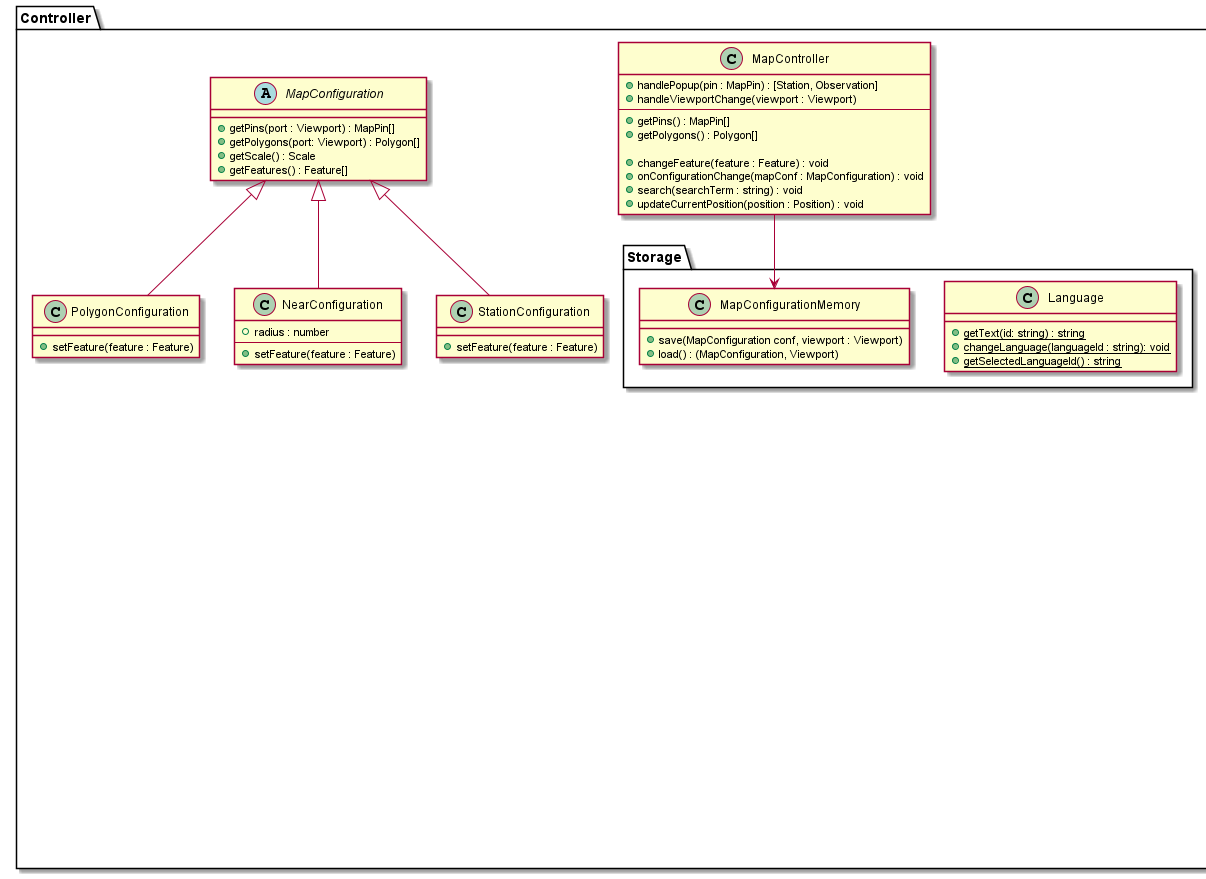
\includegraphics[angle=90, origin=c,height=\textwidth]{MVC/Controller/Controller_part1.png}
\newpage
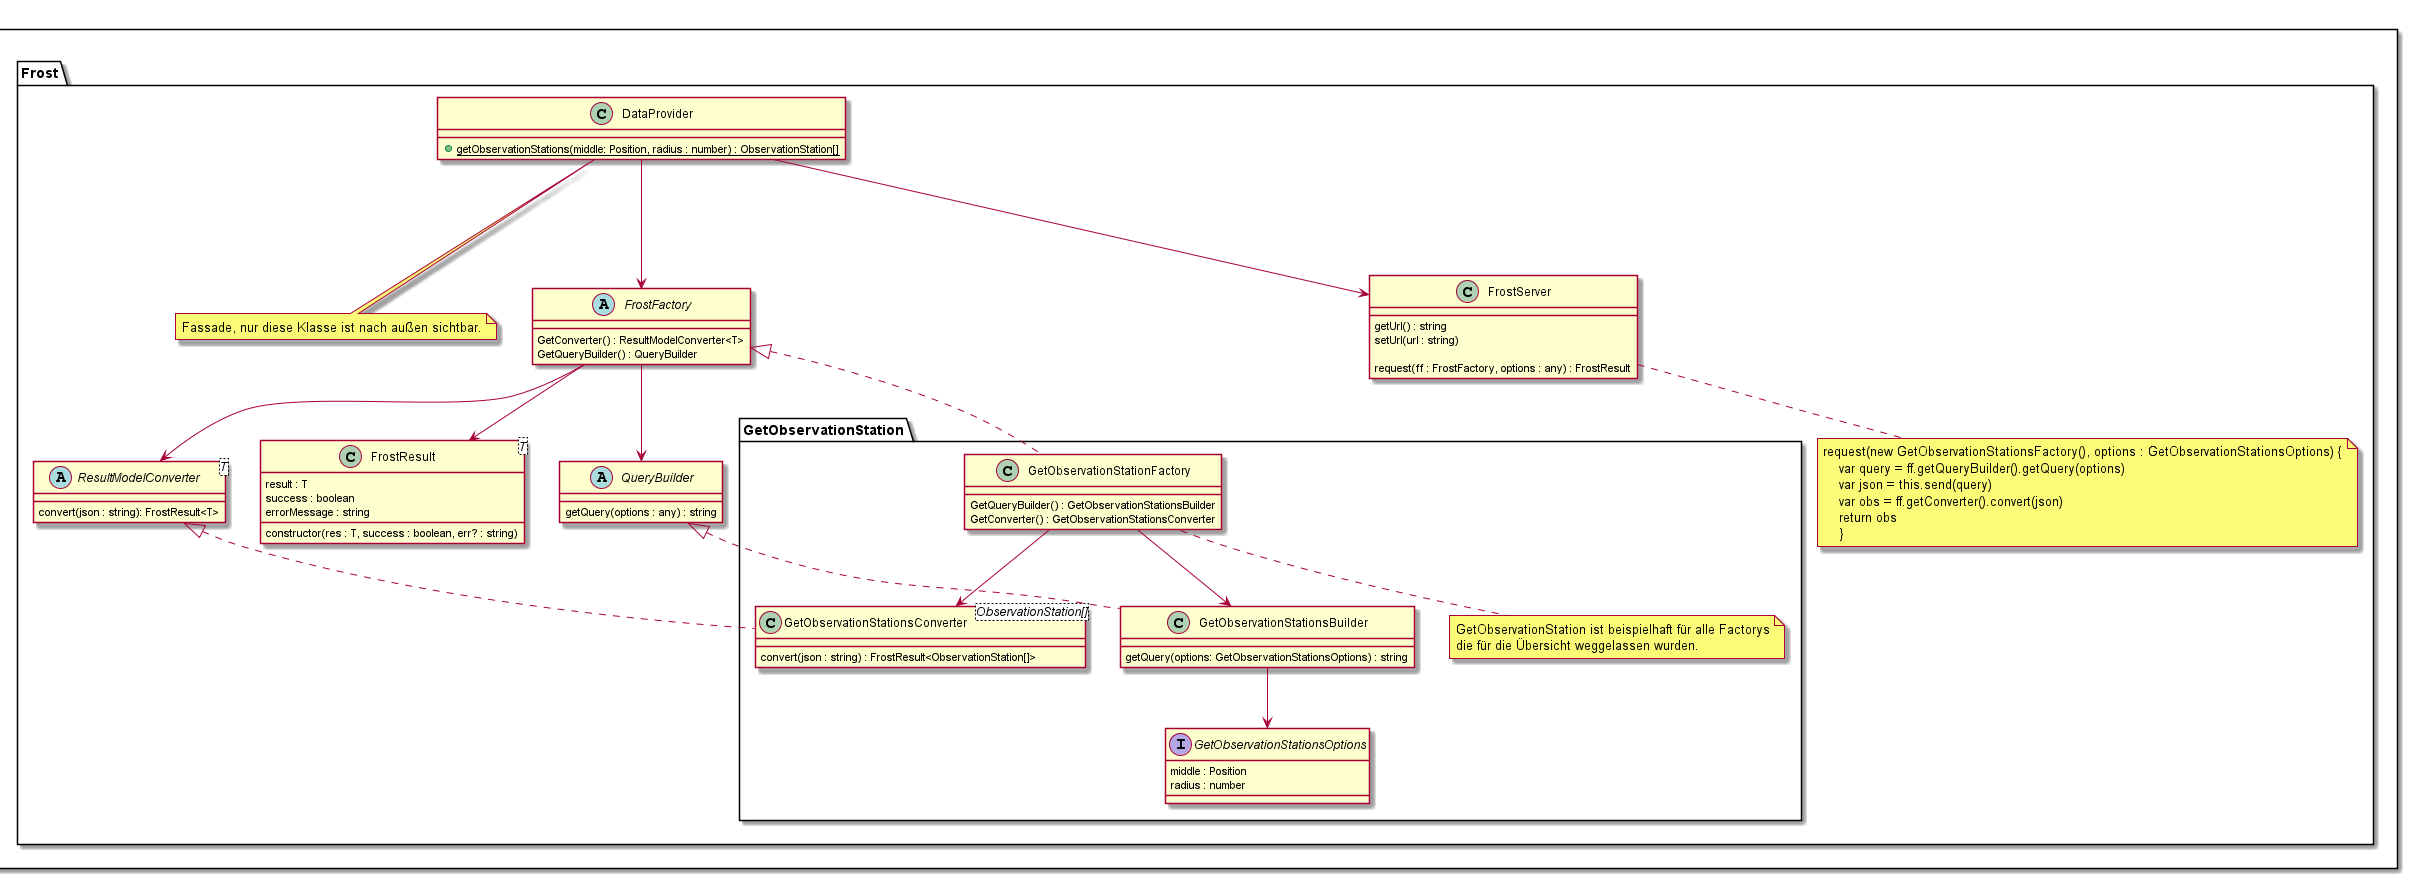
\includegraphics[angle=90, origin=c,height=\textwidth]{MVC/Controller/Controller_part2.png}

\subsubsection{FROST}

\paragraph{DataProvider / FrostServer}\mbox{}\\

\begin{Class}{DataProvider}
    Die Fassade des FROST-Namespaces. Nur mit dieser Klasse wird nach außen kommuniziert.
    Über die statischen Methoden können Anfragen an den FROST-Server gestellt werden ohne die Query oder Antwort offenzulegen.
    \textbf{Methoden}
    \begin{itemize}
        \item \texttt{<<static>> getLatestObservations(center : Position,
        \\ radius: number, feature : Feature) : Observation[]}
        \\Gibt alle Observations im spezifizierten Bereich zurück
        \item \texttt{<<static>> getLatestObservation(station : ObservationStation, feature : Feature) : Observation}
        \\ Die letzte Beobachtung der \emph{station} für das Feature \emph{feature}.
        Wenn \emph{station} \emph{feature} nicht unterstützt wird \emph{null} zurückgegeben.
        \item \texttt{<<static>> getObservations(station : ObservationStation,
        \\ start : Date, end : Date, feature : Feature) : Observation[]}
        \\ Die Beobachtungen der Station \emph{stations} für das Feature \emph{feature}
        zwischen \emph{start} und \emph{end}.
        \item \texttt{<<static>> getObservations(station : ObservationStation,
        \\ start : Date, end : Date, feature : Feature,
        \\ frequency : Frequency) : Observation[]}
        \\ Wie oben, doch gibt nur Ergebnisse im Abstand vom \emph{frequency} aus.
        \item \texttt{<<static>> getObservationStations(middle: Position,
        \\ radius : number) : ObservationStation[]}
        \\ Alle Messstationen die maximal \emph{radius} Grad Abstand von \emph{middle} haben.
        \item \texttt{<<static>> getStation(id) : ObservationStation}
        \\ Die Messstation mit Id \emph{id}.
    \end{itemize}
\end{Class}

\begin{Class}{FrostServer}
    Ein FROST-Server an den mit \emph{FrostFactory}s Anfragen gestellt werden.
    \textbf{Methoden}
    \begin{itemize}
        \item \texttt{constructor()}
        \\ Versucht die Konfigurationsdatei \emph{FrostUrl.json} zu laden und das Attribut 'url' zu lesen.
        Bei einem Fehlschlag wird ein Fehler geworfen.
        \item \texttt{getUrl() : string}
        \\ Gibt die Url des Servers zurück.
        \item \texttt{setUrl(url : string) : void}
        \\ Setzt die Url des Servers auf \emph{url}.
        \item \texttt{request(ff : FrostFactory, options : any) : FrostResult<any>}
        \\ Stellt eine Anfrage die mit \emph{ff.getQueryBuilder().getQuery(options)} erstellt wurde an den Server.
        Versucht die Antwort mit \emph{ff.getConverter().convert} in ein FrostResult<T> umzuwandeln und gibt dies zurück.
        \item \texttt{async asyncRequest(ff : FrostFactory, options : any) : Promise<FrostResult<any>>}
        \\ Wie request(ff, options) doch stellt die Anfrage asynchron.
        Dies ermöglicht ein schnelles Anzeigen der Seite während Teile noch laden (insbes. Diagramme).
    \end{itemize}
\end{Class}

\paragraph{FrostFactory}\mbox{}\\

\begin{Class}{<<abstract>> FrostFactory}
    Definiert das Erstellen einer Query und die anschließende Umwandlung der Serverantwort in Objekte des internen Models.
    \textbf{Methoden}
    \begin{itemize}
        \item \texttt{getConverter : ResultModelConverter<T>}
        \\ Eine neue Instanz eines \emph{ResultModelConverter}.
        \item \texttt{GetQueryBuilder : QueryBuilder}
        \\ Eine neue Instanz eines \emph{QueryBuilder}.
    \end{itemize}
\end{Class}

\begin{Class}{<<abstract>> QueryBuilder}
    Erstelle eine Query für einen FROST-Server mit bestimmten Optionen.
    \textbf{Methoden}
    \begin{itemize}
        \item \texttt{getQuery(options : any) : string}
        \\ Eine Query für den FrostServer mit Einstellungen aus \emph{options}.
        Angehängt an die URL des FROST-Servers + "v1.0" ergibt sich daraus die URL einer erfolgreichen Anfrage.
    \end{itemize}
\end{Class}

\begin{Class}{<<abstract>> ResultModelConverter<T>}
    Wandelt eine Antwort des FROST-Servers auf eine bestimmte Query in ein Objekt vom Typ T um.
    \textbf{Methoden}
    \begin{itemize}
        \item \texttt{convert(json : string) : FrostResult<T>}
        \\ Versucht \emph{json} in ein Objekt zu parsen und dieses Objekt in Typ T zu kopieren.
        Bei einem Fehlschlag wird ein FrostResult mit success = flase ausgegeben, sonst eines mit success = true und dem Objekt vom Typ T als result.
    \end{itemize}
\end{Class}

\paragraph{GetObservations}\mbox{}\\
\begin{Class}{GetObservationsFactory implements FrostFactory}
    \textbf{Methoden}
    \begin{itemize}
        \item \texttt{GetConverter() : GetObservationsConverter}
        \\ Eine neue Instanz eines GetObservationsConverter.
        \item \texttt{GetQueryBuilder() : GetObservationsBuilder}
        \\ Eine neue Instanz eines GetObservationsBuilder.
    \end{itemize}
\end{Class}

\begin{Class}{GetObservationsBuilder implements QueryBuilder}

    \textbf{Methoden}
    \begin{itemize}
        \item \texttt{getQuery(options : GetObservationsOptions)}
        \\ Erstellt eine FROST-Query mit folgendem Effekt:
        \\ Hole alle Observations von \emph{station} im Zeitraum \emph{start - end}
        für Feature \emph{feature}.
        \\ Wenn \emph{frequency} nicht null ist gebe nur die Observations zurück 
        die mindestens \emph{frequency} von einander entfernt sind.
    \end{itemize}
\end{Class}

\begin{Class}{GetObservationsConverter implements ResultModelConverter$\langle$Observation$\lbrack\rbrack\rangle$}

    \textbf{Methoden}
    \begin{itemize}
        \item \texttt{convert(json : string) : FrostResult<Observation[]>}
        \\ \emph{json}: Eine Antwort vom FROST-Server auf ein Query aus \emph{GetObservationsBuilder}.
        \\ Es wird versucht diese Antwort in \emph{Observation[]} umzuwandeln.
        Die Rückgabe ist dann new FrostResult(\emph{output}, true)
        \\ Schlägt dies fehl wird new FrostResult(null, false, \emph{errorMessage}) zurückgegeben.
    \end{itemize}
\end{Class}

\begin{Class}{<<interface>> GetObservationsOptions}
\begin{itemize}
    \item \texttt{station : ObservationStation}
    \item \texttt{start : Date}
    \item \texttt{end : Date}
    \item \texttt{feature : Feature}
    \item \texttt{frequency? : Frequency}
\end{itemize}
\end{Class}


\paragraph{GetLatestObservations}\mbox{}\\
\begin{Class}{GetLatestObservationsFactory implements FrostFactory}
    \textbf{Methoden}
    \begin{itemize}
        \item \texttt{GetConverter() : GetLatestObservationsConverter<Observation[]>}
        \\ Eine neue Instanz eines GetLatestObservationsConverter
        \item \texttt{GetQueryBuilder() : GetLatestObservationsBuilder}
        \\ Eine neue Instanz eines GetLatestObservationsBuilder
    \end{itemize}
\end{Class}

\begin{Class}{GetLatestObservationsBuilder implements QueryBuilder}

    \textbf{Methoden}
    \begin{itemize}
        \item \texttt{getQuery(options : GetLatestObservationsOptions)}
        \\ Erstellt eine FROST-Query mit folgendem Effekt:
        \\ Hole für alle Stationen mit Feature \emph{feature} und maximalem Abstand\emph{radius} von \emph{center}
        jeweils die neuste Observation. 
    \end{itemize}
\end{Class}

\begin{Class}{GetLatestObservationsConverter implements ResultModelConverter$\langle$Observation$\lbrack\rbrack\rangle$}

    \textbf{Methoden}
    \begin{itemize}
        \item \texttt{convert(json : string) : FrostResult<Observation[]>}
        \\ \emph{json}: Eine Antwort vom FROST-Server auf ein Query aus \emph{GetLatestObservationsBuilder}.
        \\ Es wird versucht diese Antwort in \emph{Observation[]} umzuwandeln.
        Die Rückgabe ist dann new FrostResult(\emph{output}, true)
        \\ Schlägt dies fehl wird new FrostResult(null, false, \emph{errorMessage}) zurückgegeben.
    \end{itemize}
\end{Class}

\begin{Class}{<<interface>> GetLatestObservationsOptions}
    \begin{itemize}
        \item \texttt{center : Position}
        \item \texttt{radius: number}
        \item \texttt{feature : Feature}
    \end{itemize}
\end{Class}
\paragraph{GetObservationStations}\mbox{}\\

\begin{Class}{GetObservationStationsFactory implements FrostFactory}
    \textbf{Methoden}
    \begin{itemize}
        \item \texttt{GetConverter() : GetObservationStationsConverter}
        \\ Eine neue Instanz eines GetObservationStationsConverter
        \item \texttt{GetQueryBuilder() : GetObservationStationsBuilder}
        \\ Eine neue Instanz eines GetObservationStationsBuilder
    \end{itemize}
\end{Class}

\begin{Class}{GetObservationStationsBuilder implements QueryBuilder}

    \textbf{Methoden}
    \begin{itemize}
        \item \texttt{getQuery(options : GetObservationStationsOptions)}
        \\ Erstellt eine FROST-Query mit folgendem Effekt:
        \\ Hole alle Messstationen im Radius \emph{radius} von \emph{center}.
    \end{itemize}
\end{Class}

\begin{Class}{GetObservationStationsConverter implements ResultModelConverter$\langle$ObservationStation$\lbrack\rbrack\rangle$}

    \textbf{Methoden}
    \begin{itemize}
        \item \texttt{convert(json : string) : FrostResult<ObservationStation[]>}
        \\ \emph{json}: Eine Antwort vom FROST-Server auf ein Query aus \emph{GetObservationStationsBuilder}.
        \\ Es wird versucht diese Antwort in \emph{ObservationStation[]} umzuwandeln.
        Die Rückgabe ist dann new FrostResult(\emph{output}, true)
        \\ Schlägt dies fehl wird new FrostResult(null, false, \emph{errorMessage}) zurückgegeben.
    \end{itemize}
\end{Class}

\begin{Class}{<<interface>> GetObservationStationsOptions}
    \begin{itemize}
        \item \texttt{middle : Position}
        \item \texttt{radius : number}
    \end{itemize}
\end{Class}

\begin{Class}{Converter implements ResultModelConverter}

    \textbf{Methoden}
    \begin{itemize}
        \item \texttt{convert(json : string) : FrostResult<Output>}
        \\ \emph{json}: Eine Antwort vom FROST-Server auf ein Query aus \emph{Builder}.
        \\ Es wird versucht diese Antwort in \emph{Output} umzuwandeln.
        Die Rückgabe ist dann new FrostResult(\emph{output}, true)
        \\ Schlägt dies fehl wird new FrostResult(null, false, \emph{errorMessage}) zurückgegeben.
    \end{itemize}
\end{Class}

\paragraph{GetStation}\mbox{}\\

\begin{Class}{GetStationFactory implements FrostFactory}
    \textbf{Methoden}
    \begin{itemize}
        \item \texttt{GetConverter() : GetStationConverter}
        \\ Eine neue Instanz eines GetStationConverter
        \item \texttt{GetQueryBuilder() : GetStationBuilder}
        \\ Eine neue Instanz eines GetStationBuilder.
    \end{itemize}
\end{Class}

\begin{Class}{GetStationBuilder implements QueryBuilder}

    \textbf{Methoden}
    \begin{itemize}
        \item \texttt{getQuery(options : GetStationOptions)}
        \\ Erstellt eine FROST-Query mit folgendem Effekt:
        \\ Gibt die Messstation mit Id \emph{id} zurück.
    \end{itemize}
\end{Class}

\begin{Class}{GetStationConverter implements ResultModelConverter$\langle$ObservationStation$\rangle$}

    \textbf{Methoden}
    \begin{itemize}
        \item \texttt{convert(json : string) : FrostResult<ObservationStation>}
        \\ \emph{json}: Eine Antwort vom FROST-Server auf ein Query aus \emph{GetStationBuilder}.
        \\ Es wird versucht diese Antwort in \emph{ObservationStation} umzuwandeln.
        Die Rückgabe ist dann new FrostResult(\emph{output}, true)
        \\ Schlägt dies fehl wird new FrostResult(null, false, \emph{errorMessage}) zurückgegeben.
    \end{itemize}
\end{Class}

\begin{Class}{<<interface>> GetStationOptions}
    \begin{itemize}
        \item \texttt{id : string}
    \end{itemize}
\end{Class}

\begin{Class}{Converter implements ResultModelConverter}

    \textbf{Methoden}
    \begin{itemize}
        \item \texttt{convert(json : string) : FrostResult<Output>}
        \\ \emph{json}: Eine Antwort vom FROST-Server auf ein Query aus \emph{Builder}.
        \\ Es wird versucht diese Antwort in \emph{Output} umzuwandeln.
        Die Rückgabe ist dann new FrostResult(\emph{output}, true)
        \\ Schlägt dies fehl wird new FrostResult(null, false, \emph{errorMessage}) zurückgegeben.
    \end{itemize}
\end{Class}

\iffalse
\subsubsection{FROST}

\begin{Class}{FROSTQuery}
    \textbf{Methoden}
    \begin{itemize}
        \item \texttt{send() : }
        \\Sendet die Abfrage an den Server und gibt die Antwort als QueryResult zurück.
        \item \texttt{setTop(n : int) : void}
        \\Stellt die maximale Anzahl von Objekten ein.
        \item \texttt{setSkip(n : int) : void}
        \\Stellt die Anzahl der zu überspringenden Objekte ein.
        \item \texttt{enableCount(set : boolean) : void}
        \\Stellt ein, ob die Anzahl der Objekte zurückgegeben werden soll.
        \item \texttt{setOrderBy(orderBy : string) : void}
        \\Setzt die Sortierung
        \item \texttt{setSelect(select : string) : void}
        \\Setzt die gesuchten Attribute
        \\Spezifiziert, welche Attribute in der Antwort enthalten sein sollen.
        \item \texttt{setFilter(filter : string) : void}
        \\Setzt den Filter
        \item \texttt{setExpand(expand : string) : void}
        \\Stellt ein, ob verschachtelte Objekttypen zurückgegeben werden sollen.
        \item \texttt{setId(id : string) : void}
        \\Setzt die Id des gesuchten Typs
        \item \texttt{setType(id : string) : void}
        \\Setzt den gesuchten Typ
        \item \texttt{setSubType(id : string) : void}
        \\Setzt den gesuchten Subtyp
    \end{itemize}
    Für die Standardwerte und Syntax der set-Methoden siehe: 
    \\ \url{https://fraunhoferiosb.github.io/FROST-Server/sensorthingsapi/STA-Tailoring-Responses.html}
\end{Class}

\begin{Class}{FROSTServer}
    \textbf{Methoden}
    \begin{itemize}
        \item \texttt{setUrl(url : string) : void}
        \\Setzt die URL des FROSTServers ein.
        \item \texttt{getUrl() : string}
        \\Gibt die URL des FROSTServers zurück.
    \end{itemize}
    
    \textbf{Attribute}
    \begin{itemize}
        \item \texttt{url : string}
        \\Die URL des FROSTServers.
    \end{itemize}
\end{Class}



\begin{Class}{Adapter}
    \textbf{Methoden}
    \begin{itemize}
        \item \texttt{convertToLoc(data : QueryResult) : Location[]}
        \\TODO brauchen wir diese Methode?
        \item \texttt{convertToObs(data : QueryResult,
        \\station ObservationStation) : Observations[]}
        \\Wandelt den QueryResult zu Observations um die zur gegebenen ObservationStation gehören.
        \item \texttt{convertToSta(data : QueryResult) : ObservationStation[]}
        \\Wandelt den QueryResult zu ObservationStation um. Die Position muss in der QueryResult enthalten sein.
        \item \texttt{getAvailableFeatures(date : QueryResult) : Features []}
        \\Extrahiert die verfügbaren Features (einer ObservationStation) aus dem QueryResult.
    \end{itemize}
\end{Class}

\begin{Class}{FeatureProvider}
    \textbf{Methoden}
    \begin{itemize}
        \item \texttt{getFeature(id : string)}
        \\Gibt Feature mit angegebener ID zurück. Bei erstem Aufruf werden für alle ObservedProperties vom FROSTServer Features erstellt. 
        \item \texttt{getRegisteredFeatures()}
        \\Gibt alle bekannten Features zurück.
    \end{itemize}
    \textbf{Attribute}
    \begin{itemize}
        \item \texttt{getRegisteredFeatures}
        \\Array aller bekannten Features
    \end{itemize}
\end{Class}

\fi

\subsubsection{MapPage}
\begin{Class}{MapController}
    \textbf{Methoden}
    \begin{itemize}
        \item \texttt{handlePopup(pin : MapPin) : [Station, Observation]}
        \\ Holt sich die zum \emph{pin} gehörige ObservationStation vom FROST-Server,
        holt den letzten Messwert des aktuell gewählten Features und gibt beides zurück.
        \item \texttt{handleViewportChange(viewport : Viewport)}
        \\ Aktualisiert den aktuellen Viewport auf \emph{viewport}.

        \bigskip
        \item \texttt{getPins() : MapPin[]}
        \\ Holt die Pins der aktuellen MapConfiguration mit dem aktuellen Viewport 
        und gibt sie zurück.
        \item \texttt{getPolygons() : Polygon[]}
        \\ Holt die Polygone der aktuellen MapConfiguration mit dem aktuellen Viewport 
        und gibt sie zurück.

        \bigskip
        \item \texttt{changeFeature(feature : Feature) : void}
        \\ Wechselt das aktuell gewählte Feature auf \emph{feature}.
        \item \texttt{onConfigurationChange(mapConf : MapConfiguration) : void}
        \\ Behandelt eine Änderung der Kartenkonfiguration.
        Die aktuelle Konfiguration wird auf \emph{mapConf} gesetzt und die Pins und Polygone der Karte aktualisiert.
        \item \texttt{search(searchTerm : string) : void}
        \\ Versucht den \emph{searchTerm} als Position zu interpretieren und setzt die Mitte des Viewports darauf.
        Wenn die Interpretation nicht möglich ist wird eine Warnung ausgegeben.
        \item \texttt{updateCurrentPosition(position : Position) : void}
        \\ Setzt die aktuelle Position auf \emph{position} und aktualisiert die Karte.
    \end{itemize}
\end{Class}

\begin{Class}{MapConfiguration}
    \textbf{Methoden}
    \begin{itemize}
        \item \texttt{getPins(port : Viewport) : MapPin[]}
        \\ Holt Messstationen die eines der gewählten Features unterstützen und im \emph{viewport} liegen vom Server,
        erstellt daraus MapPins und gibt sie zurück.
        \item \texttt{getPolygons(port: Viewport) : Polygon[]}
        \\ Wie getPins(v), nur mit Polygonen. 
        \item \texttt{getScale() : Scale}
        \\ Gibt die aktuell aktive Skala zurück.
        \item \texttt{getFeatures() : Feature[]}
        \\ Die aktuell gewählten Features die von der Konfiguration benötigt werden.
    \end{itemize}
\end{Class}

\begin{Class}{StationConfiguration extends MapConfiguration}
    Eine Konfiguration bei der die einzelnen Messstationen als Marker dargestellt werden.
    \textbf{Methoden}
    \begin{itemize}
        \item \texttt{getPins(port : Viewport) : MapPin[]}
        \\ Messstationen, als Pins repräsentiert.
        erstellt daraus MapPins und gibt sie zurück.
        \item \texttt{getPolygons(port: Viewport) : Polygon[]}
        \\ Gibt [] zurück.
        \bigskip
        \item \texttt{setFeature(feature : Feature)}
        \\ Setzt die gewählten Features auf [\emph{feature}].
    \end{itemize}
\end{Class}

\begin{Class}{PolygonConfiguration extends MapConfiguration}
    \textbf{Methoden}
    \begin{itemize}
        \item \texttt{getPins(port : Viewport) : MapPin[]}
        \\ Gibt [] zurück.
        erstellt daraus MapPins und gibt sie zurück.
        \item \texttt{getPolygons(port: Viewport) : Polygon[]}
        \\ Spannt zwischen jeweils drei Stationen Polygone auf.
        Die Polygone werden in der Farbe gefärbt die entsprechend der Skala für den Mittelwert der einzelnen letzten Messwerte entsprechen.
        \bigskip
        \item \texttt{setFeature(feature : Feature)}
        \\ Setzt die gewählten Features auf [\emph{feature}].
    \end{itemize}
\end{Class}

\begin{Class}{NearConfiguration extends MapConfiguration}
    \textbf{Methoden}
    \begin{itemize}
        \item \texttt{getPins(port : Viewport) : MapPin[]}
        \\ Die Messstationen werden als Pins repräsentiert die entsprechend der Skala gefärbt sind.
        \\ Dabei wird allerdings der Messwert so skaliert dass der niedrigste Messwert im Radius 0 ist, der höchste die größte Zahl der Skala.
        erstellt daraus MapPins und gibt sie zurück.
        \item \texttt{getPolygons(port: Viewport) : Polygon[]}
        \\ Gibt [] zurück.
        \bigskip
        \item \texttt{setFeature(feature : Feature)}
        \\ Setzt die gewählten Features auf [\emph{feature}].
    \end{itemize}
    \textbf{Attribute}
    \begin{itemize}
        \item \texttt{Radius}
        \\ Der Radius aus dem die Daten für die Skalierung geholt werden.
    \end{itemize}
\end{Class}

\subsubsection{Storage}

\begin{Class}{Language}
    \textbf{Methoden}
    \begin{itemize}
        \item \texttt{<<static>> getText(id : string) : string}
        \\ Gibt den Text mit der Id \emph{id} in der gewählten Sprache zurück.
        \item \texttt{<<static>> changeLanguage(lang : string)}
        \\ Lädt die Sprache mit der Id \emph{lang} und wählt sie aus.
        \item \texttt{<<static>> getSelectedLanguageId() : string}
        \\ Die Id der aktuell gewählten Sprache.
    \end{itemize}

\end{Class}


\begin{Class}{MapConfigurationMemory}
    \textbf{Methoden}
    \begin{itemize}
        \item \texttt{save(MapConfiguration conf, viewport : Viewport)}
        \\ Speichert die aktuelle MapConfiguration und Viewport im localStorage unter der ID 'mapConf'
        \item \texttt{load() : (MapConfiguration, Viewport)}
        \\ Lädt das Tupel aus localStorage mit Id 'mapConf' und gibt es zurück.
        \\ Gibt eine neue MapConfiguration und Viewport mit Standardwerten zurück wenn 
        dieser Eintrag nicht existiert.
    \end{itemize}

\end{Class}